\documentclass[tikz,border=2pt]{standalone}
\usepackage{amsmath,amssymb}
\usepackage{tikz}
\usetikzlibrary{matrix,arrows.meta}

\begin{document}
% Minimum zero cover of the reduced matrix: the five zeros can be covered by row 2 and column
% 2 (two lines), fewer than n = 3, so no complete zero assignment exists yet.
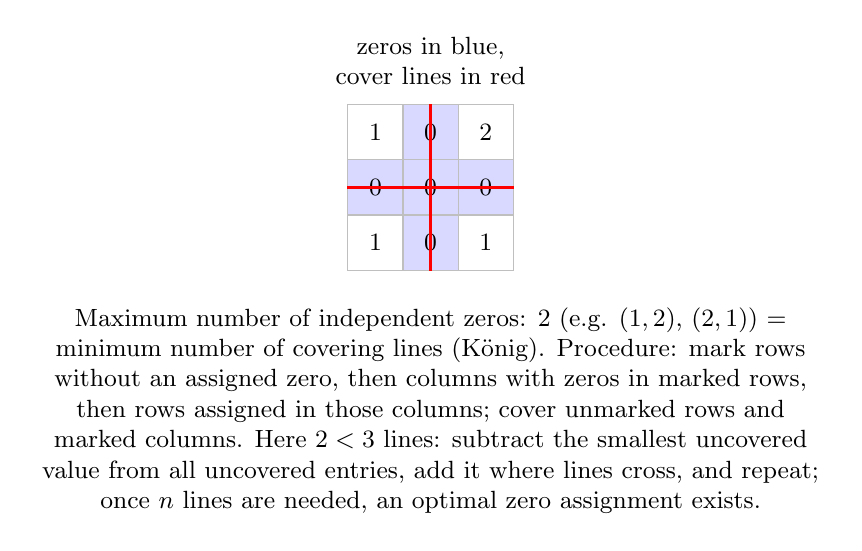
\begin{tikzpicture}[every node/.style={font=\small}, >={Latex[length=1.8mm]}]
	\matrix (Cm) [matrix of math nodes, nodes={minimum size=7mm, anchor=center, draw=gray!50}, column sep=-\pgflinewidth, row sep=-\pgflinewidth] at (0,0) {1 & |[fill=blue!15]| 0 & 2 \\ |[fill=blue!15]| 0 & |[fill=blue!15]| 0 & |[fill=blue!15]| 0 \\ 1 & |[fill=blue!15]| 0 & 1 \\};
	\draw[red, very thick] (Cm-2-1.west) -- (Cm-2-3.east);
	\draw[red, very thick] (Cm-1-2.north) -- (Cm-3-2.south);
	\node[anchor=south, font=\small, align=center] at (Cm.north) {zeros in blue,\\ cover lines in red};
		\node[anchor=north, align=flush center, text width=10cm] at (0,-1.4) {Maximum number of independent zeros: $2$ (e.g. $(1,2)$, $(2,1)$) $=$ minimum number of covering lines (K\"onig). Procedure: mark rows without an assigned zero, then columns with zeros in marked rows, then rows assigned in those columns; cover unmarked rows and marked columns. Here $2<3$ lines: subtract the smallest uncovered value from all uncovered entries, add it where lines cross, and repeat; once $n$ lines are needed, an optimal zero assignment exists.};
\end{tikzpicture}
\end{document}
